\documentclass{standalone}%

%% Language and font encodings
%\usepackage[english]{babel}
%\usepackage[utf8x]{inputenc}
%\usepackage[T1]{fontenc}

%% Sets page size and margins
%\usepackage[a4paper,top=3cm,bottom=2cm,left=1cm,right=1cm,marginparwidth=1.75cm]{geometry}

\usepackage[dvipsnames]{xcolor}

%% Useful packages
\usepackage{amsmath}
\usepackage{graphicx}
\usepackage[colorinlistoftodos]{todonotes}
\usepackage[colorlinks=true, allcolors=blue]{hyperref}





%\usepackage{xcolor}

%% tikz packages
\usepackage{tikz,pgf}
\usetikzlibrary{trees}
\usetikzlibrary{backgrounds}
\usepackage{tikz-dependency}



\usetikzlibrary{decorations.pathreplacing}

\definecolor{my_green}{rgb}{0, 0.6, 0.5}
\definecolor{my_orange}{rgb}{0.9, 0.6, 0}
\definecolor{my_purple}{rgb}{0.8, 0.6, 0.7}
\definecolor{my_blue}{rgb}{0, 0.45, 0.7}

\tikzstyle{bag} = [align=center]

\begin{document}



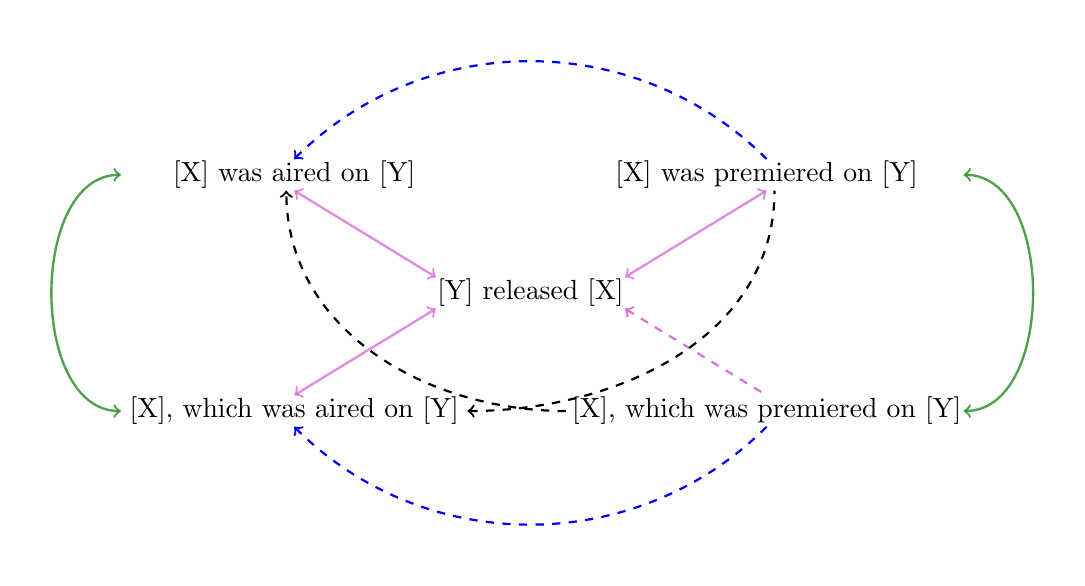
\begin{tikzpicture}[
  emb/.style={rectangle,draw,fill=white,minimum width=2cm,minimum height=0.6cm,rounded corners=.8ex},
  normal/.style={rectangle,draw,fill=white,minimum width=4cm,minimum height=0.8cm,rounded corners=.8ex},
  path_embedding/.style={rectangle,draw,fill=blue!20,minimum width=4cm,    minimum height=0.7cm},
  nc_embedding/.style={rectangle,draw,fill=orange!50,minimum width=2.5cm,    minimum height=0.7cm},
  word_embedding/.style={rectangle,draw,fill=my_green!40,minimum width=2.5cm,    minimum height=0.7cm},
  every neuron_empty/.style={circle,draw,minimum size=0.2cm},
  every neuron/.style={circle,draw,fill=orange!50,minimum size=0.2cm},
  every neuron1/.style={circle,draw,fill=orange!50,minimum size=0.2cm},
  every neuron2/.style={circle,draw,fill=blue!50,minimum size=0.2cm},
  every neuron3/.style={circle,draw,fill=green!50,minimum size=0.2cm},
  every neuron4/.style={circle,draw,fill=green!50,minimum size=0.2cm},
  every neurontar/.style={circle,draw,fill=brown!50,minimum size=0.5cm},
  every text-box/.style={rectangle,minimum size=0.6cm},
  every rect/.style={rectangle,draw,fill=gray!50,minimum size=0.6cm},
  every vecrec/.style={rectangle,draw,fill=none,minimum width=1.5cm, minimum height=0.8cm},
  every oper/.style={rectangle,draw,fill=red!50,minimum size=0.5cm},
  every oper2/.style={rectangle,draw,fill=pink!50,minimum size=0.5cm},
  neuron missing/.style={draw=none,fill=none,scale=2,execute at begin node=\color{black}$\cdots$}
  ]
  
  	

    
\newcommand\mystring{{"The","dog","ran"}}

% text
\node[] at (0,0) {[Y] released [X]};
\node[] at (-3,1.5) {[X] was aired on [Y]};
\node[] at (3,1.5) {[X] was premiered on [Y]};
\node[] at (-3,-1.5) {[X], which was aired on [Y]};
\node[] at (3,-1.5) {[X], which was premiered on [Y]};

\path[draw,<->, opacity=0.8, line width=0.3mm, color=Orchid] (-1.2, 0.2) to (-3, 1.3);
\path[draw,<->, opacity=0.8, line width=0.3mm, color=Orchid] (1.2, 0.2) to (3, 1.3);
\path[draw,<->, opacity=0.8, line width=0.3mm, color=Orchid] (-1.2, -0.2) to (-3, -1.3);
\draw[<-,thick,Orchid,dashed] (1.2, -0.2) to (3, -1.3); node[anchor=west];


% horizontal
\draw[<-,thick,blue,dashed] (-3, 1.7) to [out=45,in=135] (3, 1.7); node[anchor=west];
\draw[<-,thick,blue,dashed] (-3, -1.7) to [out=-45,in=-135] (3, -1.7); node[anchor=west];


% vertical
\path[draw,<->, opacity=0.8, line width=0.3mm, color=ForestGreen] (-5.2, 1.5) to [out=180,in=180] (-5.2, -1.5);
\path[draw,<->, opacity=0.8, line width=0.3mm, color=ForestGreen] (5.5, 1.5) to [out=0,in=0] (5.5, -1.5);


% diagonal
\draw[->,thick,black,dashed] (0.45, -1.5) to [out=-180,in=-90] (-3.1, 1.3); node[anchor=west];
\draw[<-,thick,black,dashed] (-0.8, -1.5) to [out=0,in=-90] (3.1, 1.3); node[anchor=west];



\end{tikzpicture}

\end{document}